\documentclass[11pt,a4paper]{article}
\usepackage[utf8]{inputenc}
\usepackage[T1]{fontenc}
\usepackage{lmodern}
\usepackage[french]{babel}
\usepackage[margin=2.1cm]{geometry}
\usepackage{microtype}
\usepackage{amsmath,amssymb}
\usepackage{booktabs}
\usepackage{array}
\usepackage[table]{xcolor}
\usepackage{graphicx}
\usepackage{caption}
\usepackage[most]{tcolorbox}
\definecolor{navy}{HTML}{1F3864}
\definecolor{bluemid}{HTML}{2E5496}
\definecolor{lightblue}{HTML}{D6E0F0}
\captionsetup{font=small,labelfont={bf,color=navy},labelsep=period}
\graphicspath{{../figures/}}
\newtcolorbox{cle}[1][]{colback=lightblue!40,colframe=navy,boxrule=0.6pt,
  arc=2pt,left=8pt,right=8pt,top=6pt,bottom=6pt,#1}

\title{\vspace{-1.2cm}\color{navy}\bfseries Validation et adéquation du socle\\[2pt]
  \large La sévérité GPD et la fréquence NB passent les tests}
\author{Kélian Kaddouri}
\date{27 juillet 2026}

\begin{document}
\maketitle
\vspace{-0.9cm}

\begin{cle}
\textbf{La question.} Avant d'agréger, les lois posées s'ajustent-elles vraiment aux données~?
Un jury actuariel le cherche en premier. On teste les deux briques qui portent le SCR, sans
complaisance.
\end{cle}

\medskip
\begin{center}
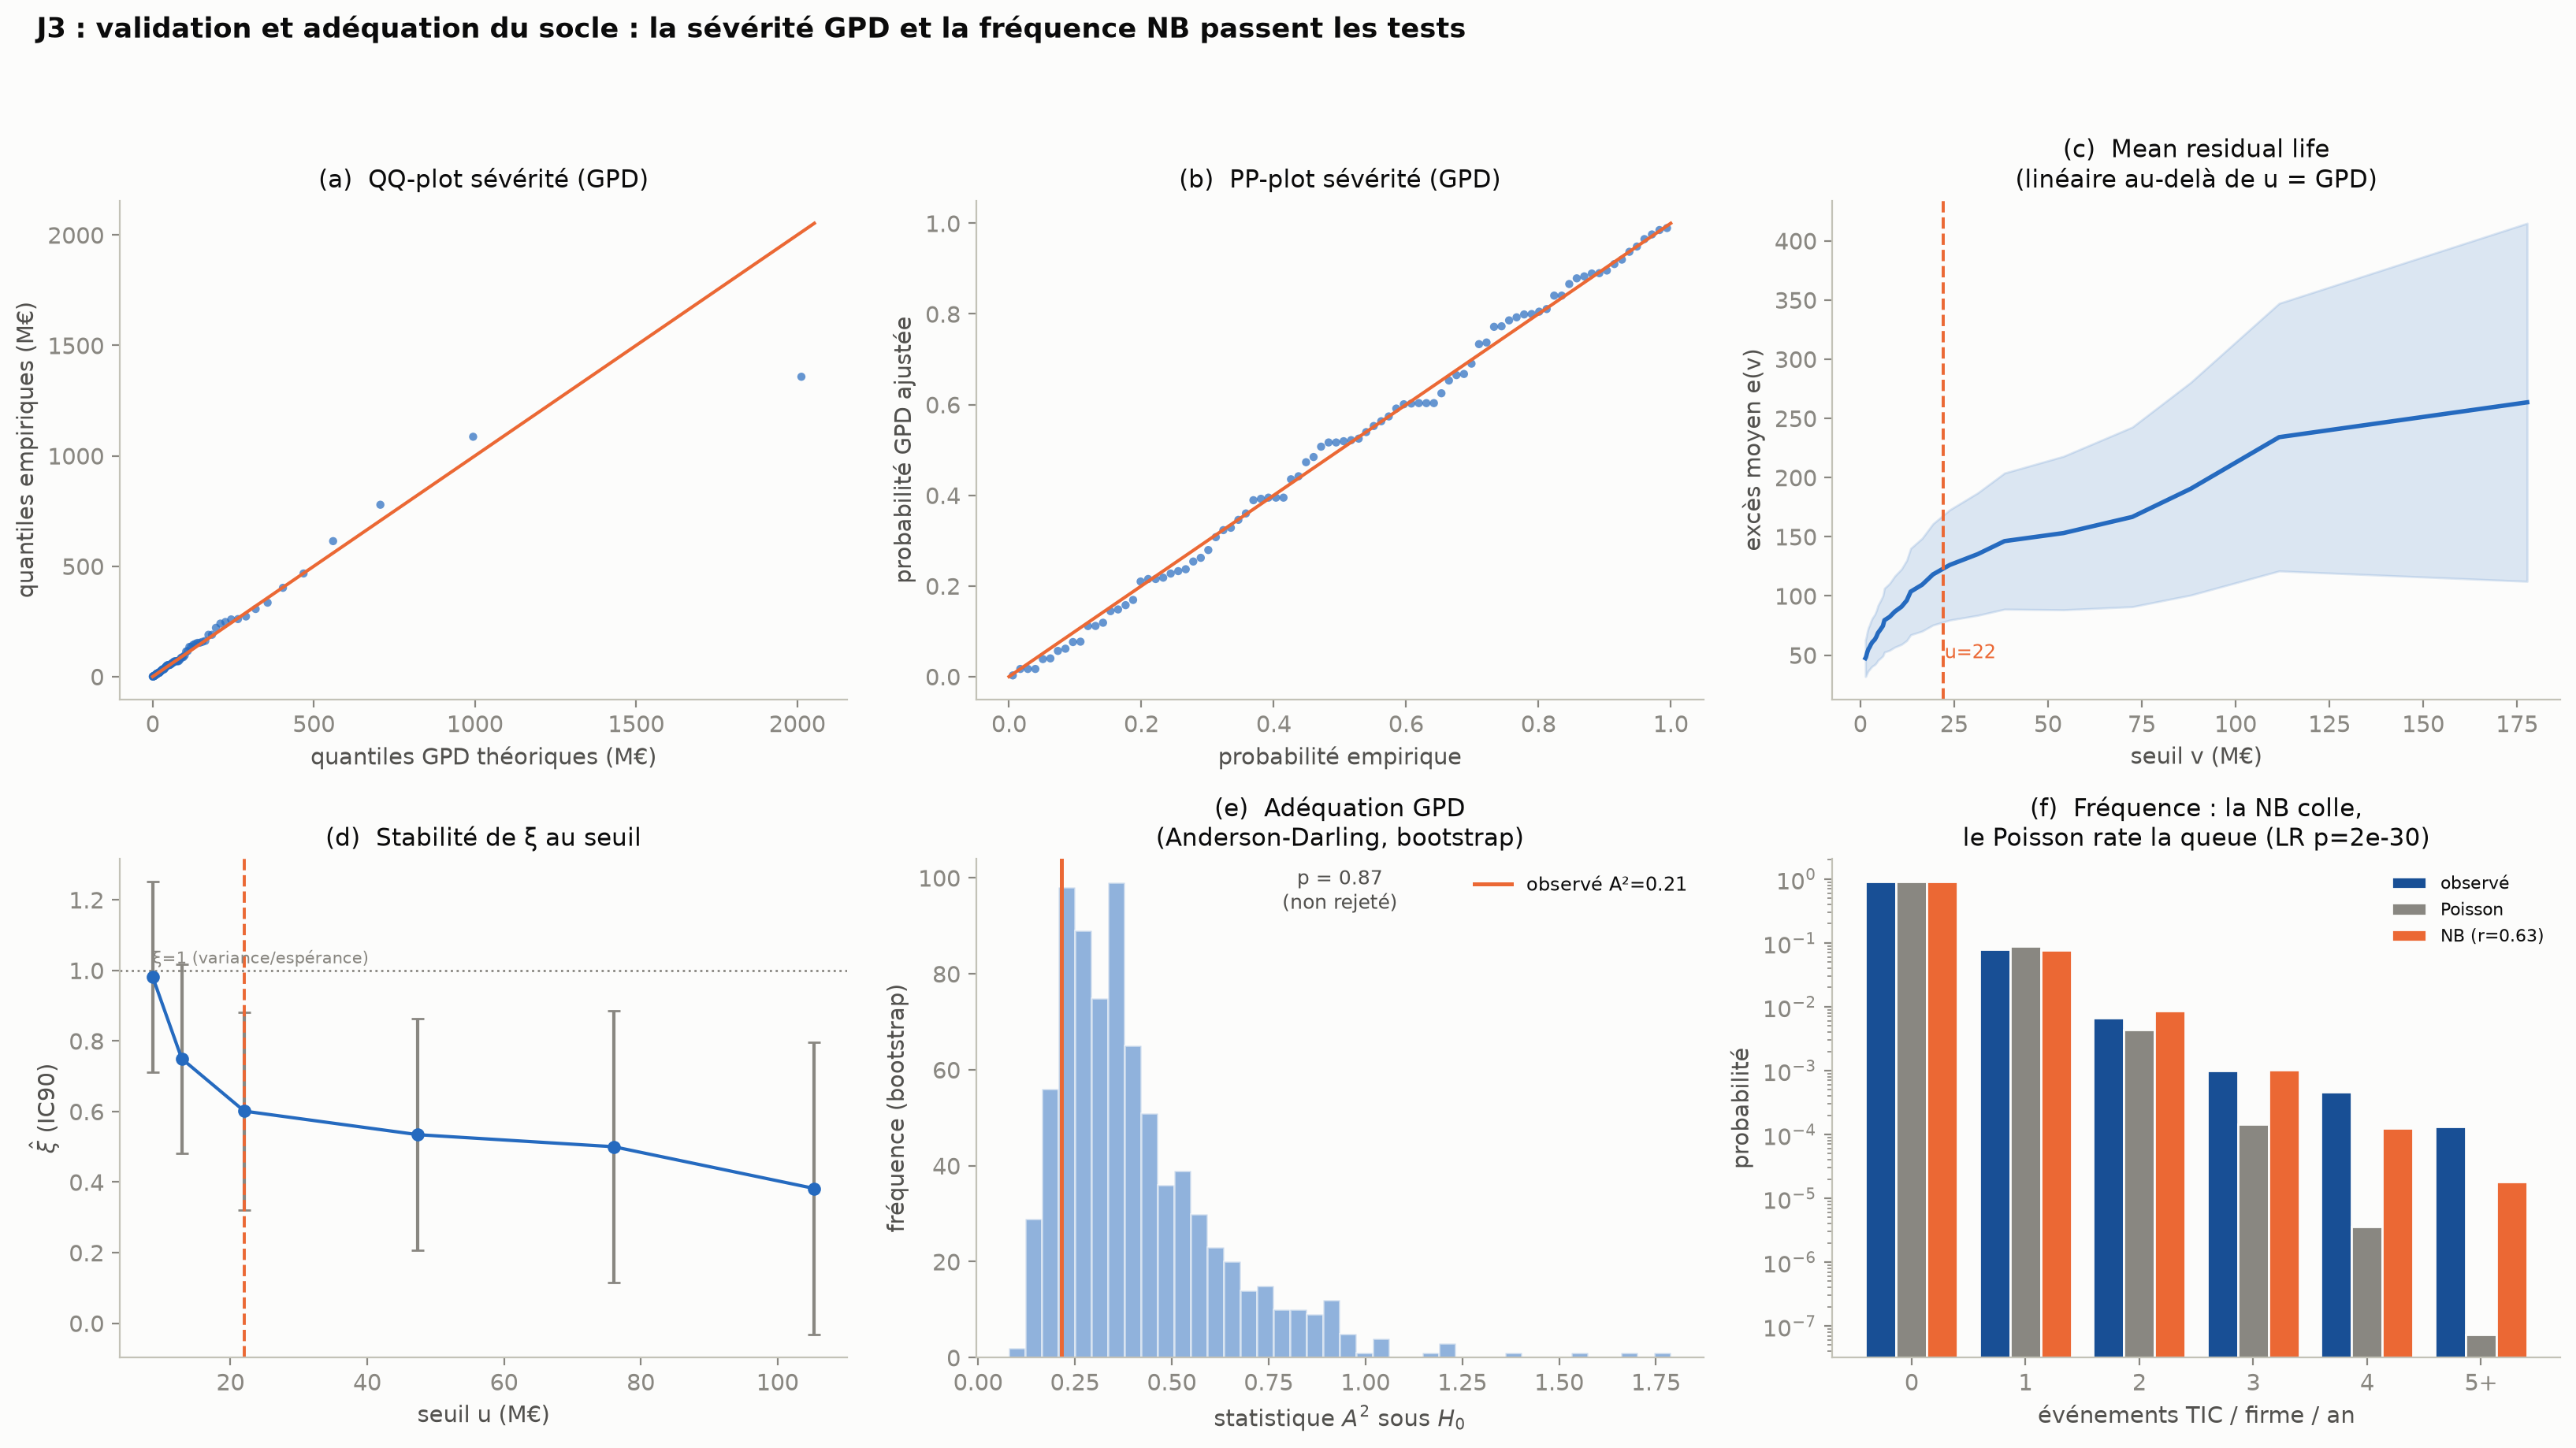
\includegraphics[width=\linewidth]{J3_validation_adequation.png}
\captionof{figure}{\textbf{(a-b)} QQ-plot et PP-plot de la sévérité contre la GPD ajustée.
\textbf{(c)} vie résiduelle moyenne, linéaire au-delà de $u$. \textbf{(d)} stabilité de
$\hat\xi$ au seuil. \textbf{(e)} test d'Anderson-Darling, loi nulle par bootstrap paramétrique.
\textbf{(f)} adéquation de la fréquence, la NB contre le Poisson.}
\end{center}

\noindent\textbf{Sévérité (GPD).} Elle passe les diagnostics sans réserve. Les tracés
quantile-quantile et probabilité-probabilité s'alignent sur la diagonale ; la vie résiduelle
moyenne est linéaire au-delà du seuil (signature GPD) ; $\hat\xi$ reste stable autour de
$0{,}60$. Les tests formels ne rejettent pas l'ajustement, avec une $p$-value obtenue par
\textbf{bootstrap paramétrique} (les valeurs critiques tabulées ne valent pas quand les
paramètres sont estimés) : Anderson-Darling $p=0{,}87$, Kolmogorov-Smirnov $p=0{,}87$. Enfin, la
\textbf{couverture réelle} de l'intervalle de confiance à $90\,\%$ de $\xi$, mesurée par
simulation à $n$ fini, vaut $86\,\%$ : proche du nominal.

\medskip
\noindent\textbf{Fréquence (NB).} Sur les $14\,944$ cellules firme-année du panel financier, la
binomiale négative domine le Poisson sans ambiguïté : le test du rapport de vraisemblance donne
$p\approx 10^{-30}$. La surdispersion ($\mathrm{Var}/\mathbb{E}=1{,}19$, $r=0{,}63$) est un
\emph{fait}, non un artefact.

\begin{cle}
\textbf{Ce que la validation établit, et ce qu'elle n'établit pas.} Les tests portent sur la
\textbf{forme} des lois, pas sur le \emph{niveau} du capital : ils confirment que la GPD et la
NB sont les bons objets, mais laissent entière l'incertitude sur $\xi$ et donc sur la VaR.
Adéquation n'est pas certitude : c'est précisément pourquoi le SCR se lit en intervalle.
\end{cle}

\smallskip
\noindent\footnotesize\textcolor{navy}{\textbf{Source.}} Script
\texttt{1\_fondations/47\_validation\_adequation.py}, figure \texttt{J3\_validation\_adequation.png}.
Calibration OpRisk cyber\,$\times$\,finance (POT, $u=$ percentile 85).

\end{document}
